\documentclass[english,compress]{beamer}
\usepackage{kloeckislides}
\nonstopmode

\usepackage[normalem]{ulem}
\usepackage{pifont}
\usepackage{ifthen}

\setbeamercolor{section in head/foot}{use=structure,bg=structure.fg!25!bg}
\defbeamertemplate*{footline}{split theme}
{%
  \leavevmode%
  \begin{beamercolorbox}[wd=.5\paperwidth,ht=2.5ex,dp=1.125ex]{section in head/foot}%
    \insertsectionnavigationhorizontal{\paperwidth}{\hskip0pt plus1filll}{}%
  \end{beamercolorbox}%
  %\begin{beamercolorbox}[wd=.5\paperwidth,ht=2.5ex,dp=1.125ex]{subsection in head/foot}%
    %\insertsubsectionnavigationhorizontal{.5\paperwidth}{}{\hskip0pt plus1filll}%
  %\end{beamercolorbox}%
}


%\useoutertheme[subsection=false]{miniframes}

\setbeamertemplate{frametitle}[default][center]

\AtBeginDocument{%
  {
    \usebeamercolor{section in head/foot}
  }
  
  \pgfdeclareverticalshading{beamer@headfade}{\paperwidth}
  {%
    color(0cm)=(bg);
    color(1.25cm)=(section in head/foot.bg)%
  }

  \setbeamercolor{section in head/foot}{bg=}
}

\addtoheadtemplate{\pgfuseshading{beamer@headfade}\vskip-1.25cm}{}

\beamertemplatedotitem

\setbeamercolor{section in head/foot}{parent=palette quaternary}
\setbeamercolor{subsection in head/foot}{parent=palette primary}

\setbeamercolor{author in head/foot}{parent=section in head/foot}
\setbeamercolor{title in head/foot}{parent=subsection in head/foot}



\AtBeginSection[] {
  \begin{frame}<beamer>
  \frametitle{Outline}
  \tableofcontents[sectionstyle=show/shaded,subsectionstyle=show/show/hide]
\end{frame}
}
\AtBeginSubsection[] {
  \begin{frame}<beamer>
  \frametitle{Outline}
  \tableofcontents[sectionstyle=show/shaded,subsectionstyle=show/shaded/hide]
\end{frame}
}

\newcommand{\technicality}[2]{%
  {\strut #1\\
    \begin{beamercolorbox}[sep=1mm]{block body}
      #2
    \end{beamercolorbox}
  }%
}

\lstset{
  language=C++,
  rangebeginprefix=//\ ,
  rangeendprefix=//\ ,
}

\def\weblink#1#2{\href{#1}{\color{blue}\underline{#2}}}

\definecolor{fetch}{RGB}{227,110,35}
\definecolor{alu}{RGB}{255,188,24}
\definecolor{context}{RGB}{132,146,175}

\usepackage{keystroke}

\setbeamertemplate{navigation symbols}{}


\begin{document}
% {{{ front matter

\title{High-Performance Scientific Computing\\Lecture 6: MPI}

\date{MATH-GA 2011 / CSCI-GA 2945 $\cdot$ October 10, 2012}

\frame{\titlepage}

\begin{frame}{Today}
  \tableofcontents[hideallsubsections]
\end{frame}
% }}}
% -----------------------------------------------------------------------------
\begin{frame}{Bits and pieces}
  \begin{itemize}
    \item HW2: \dots
    \item HW4: due today
    \item HW5: out tomorrow
    \item On HW5: 5 minute project pitch $\rightarrow$ due next week!
    \item Project: form teams
  \end{itemize}
\end{frame}
% -----------------------------------------------------------------------------
\begin{frame}[fragile]{Atomic: Compare-and-swap}
  \begin{lstlisting}
  int atomic_cmpxchg (__global int *p, int cmp, int val)
  int atomic_cmpxchg (__local int *p, int cmp, int val)
  \end{lstlisting}

  Does:
  \begin{itemize}
    \item Read the 32-bit value (referred to as
    old) stored at location pointed by p.
  \item Compute \texttt{(old == cmp) ? val : old}.
  \item Store result at location pointed by p.
  \item Returns old.
  \end{itemize}
  \uncover<2>{
    \begin{tikzpicture} [overlay]
      \node [above left=1cm of current page.south east, draw,drop shadow,fill=white,
      inner xsep=0.5cm,inner ysep=0.5cm,thick]
        {
          Implement atomic \texttt{float} add?
        } ;
    \end{tikzpicture}
  }
\end{frame}
% -----------------------------------------------------------------------------
\section{Tool of the day: gdb}
% -----------------------------------------------------------------------------
\begin{frame}{Git}
  \begin{center}
  \Huge Demo time
  \end{center}
\end{frame}
% -----------------------------------------------------------------------------
\section{MPI: Point-to-Point}
% -----------------------------------------------------------------------------
% {{{
% -----------------------------------------------------------------------------
\begin{frame}{MPI}
  \begin{center}
  \Huge Demo time
  \end{center}
\end{frame}
% -----------------------------------------------------------------------------
\def\hilite<#1>#2{\alt<#1>{\colorbox{blue!30}{#2}}{\colorbox{white}{#2}}%
}
\begin{frame}{Send definition}
  \textbf{MPI 3.0, Section 3.4:}

  \uncover<+>{}
  \begin{quote}
    \upshape
    [\texttt{MPI\_Send}] is \hilite<+->{blocking}: it does not
    return until the message data and envelope have been safely stored
    away so that the sender is \hilite<+->{free to modify the send buffer}.
  \end{quote}
\end{frame}
% -----------------------------------------------------------------------------
\begin{frame}{Send definition}
  \textbf{MPI 3.0, Section 3.4, more:}

  \uncover<+>{}
  \medskip
  \begin{quote}
    \upshape
    [\texttt{MPI\_Send}] uses the
    \hilite<+->{standard
    \tikz \coordinate (cmode) ;
    communication mode}. In this mode, it is up to
    MPI to decide whether outgoing messages will be buffered.

    \medskip
    MPI
    \tikz \coordinate (may) ;
    \hilite<+->{may} buffer outgoing messages.
    In such a case, the send call may complete before a matching
    receive is invoked. On the other hand, MPI may choose not to
    buffer outgoing messages.
  \end{quote}
  \uncover<+->{
    \begin{tikzpicture} [overlay]
      \node [
        above right=1cm of current page.south west, draw,drop shadow,fill=white,
        inner sep=5mm,thick, text width=0.3\textwidth] (may-descr)
        {
          What is correct behavior?

          \medskip
          Must, should, may (RFC 2119)
        } ;
        \draw [ultra thick,->] (may-descr) -- ($(may)+(2ex,0)$) ;
    \end{tikzpicture}
  }
  \uncover<+->{
    \begin{tikzpicture} [overlay]
      \node [
        above left=5mm of current page.south east, draw,drop shadow,fill=white,
        inner sep=5mm,thick, text width=0.4\textwidth] (cmode-descr)
        {
          Alternative communication modes:
          \begin{itemize}
            \item Buffered
            \item Synchronous
            \item Ready
          \end{itemize}
        } ;
        \draw [ultra thick,->] (cmode-descr) -- (cmode) ;
    \end{tikzpicture}
  }
\end{frame}
% -----------------------------------------------------------------------------
\begin{frame}{Send definition}
  \textbf{MPI 3.0, Section 3.4, yet more:}

  \uncover<+>{}
  \begin{quote}
    \upshape
    A send in standard mode can be \hilite<+->{started} whether or not a matching
    receive has been \hilite<+->{posted}. 

    \medskip
    It may \hilite<+->{complete} before a
    \hilite<+->{matching} receive is posted.

    \medskip
    The standard mode send is \hilite<+->{non-local}: successful
    completion of the send operation may depend on the occurrence of a
    matching receive.
  \end{quote}
\end{frame}
% -----------------------------------------------------------------------------
\begin{frame}{Meta-lesson}
  \begin{center}
    \Large
    Can learn a lot from \emph{how} something is said.
  \end{center}
\end{frame}
% -----------------------------------------------------------------------------
\begin{frame}{Lessons}
  \begin{itemize}
    \item Blocking $\leftrightarrow$ buffers
    \item Communication modes
    \item Operation life cycle
    \item Matching
    \item Non-locality
  \end{itemize}
\end{frame}
% -----------------------------------------------------------------------------
\begin{frame}{Removing the deadlock}
  Two ways laid out:
  \pause
  \begin{itemize}
    \item Use buffered send (brittle!)
    \item Change order (not always easy! Example?)
  \end{itemize}
  \pause
  \bigskip
  Would like a middle ground: 
  \begin{quote}
  ``Just keep the buffer I've got right here!''
  \end{quote}
  But when is it safe to reuse that buffer?
\end{frame}
% -----------------------------------------------------------------------------
\begin{frame}{Non-blocking}
  \textbf{MPI 3.0, Section 3.5:}
  \begin{quote}
    \upshape
    Nonblocking message-passing operations [...] can be used to avoid
    the need for buffering outgoing messages.
  \end{quote}
  Additional Advantage: \textbf{[Sec. 3.7]}
  \begin{quote}
    \upshape
    One can improve performance on many systems by overlapping
    communication and computation.
  \end{quote}
  \uncover<+>{}
  \uncover<+->{
    \begin{tikzpicture} [overlay]
      \node [above left=0.5cm of current page.south east, draw,drop shadow,fill=white,
      inner xsep=0.5cm,inner ysep=0.5cm,thick,text width=0.6\textwidth]
        {
          Nonblocking can be \emph{combined} with
          buffered/ready/synchronous.

          $\rightarrow$ It's not a ``mode''.

          \bigskip
          Nonblocking sends can be matched with blocking receives, and
          vice-versa. \textbf{[3.7]}
        } ;
    \end{tikzpicture}
  }
\end{frame}
% -----------------------------------------------------------------------------
\begin{frame}{MPI}
  \begin{center}
  \Huge Nonblocking demo time
  \end{center}
\end{frame}
% -----------------------------------------------------------------------------
\begin{frame}{Partitioning for neighbor communication}
  \begin{center}
    \includegraphics[height=7cm]{mesh-partition.png}
  \end{center}
  \uncover<+>{}
  \uncover<+->{
    \begin{tikzpicture} [overlay]
      \node [above left=0.5cm of current page.south east, draw,drop shadow,fill=white,
      inner xsep=0.5cm,inner ysep=0.5cm,thick]
        {
          How can I chop up a domain?
        } ;
    \end{tikzpicture}
  }
\end{frame}
% -----------------------------------------------------------------------------
\begin{frame}{MPI}
  \begin{center}
  \Huge Neighbor comm demo time
  \end{center}
\end{frame}
% -----------------------------------------------------------------------------
\begin{frame}{MPI: Ordering}
  \uncover<+->{}
  \textbf{MPI 3.0, Section 3.5:}
  \begin{quote}
    \upshape
    \textbf{Order} Messages are \hilite<+->{non-overtaking}: If a
    sender sends two messages in succession to the same destination,
    and both match the same receive, then this operation cannot
    receive the second message if the first one is still pending.

    \bigskip
    If a receiver posts two receives in succession,
    and both match the same message, then the second receive operation
    cannot be satisfied
    by this message, if the first one is still pending.
  \end{quote}
\end{frame}
% -----------------------------------------------------------------------------
\begin{frame}[fragile]{MPI: More on Ordering}
  Possible problem?
  \begin{lstlisting}
    if (rank == 0)
    {
      MPI_Bsend(buf1, count, MPI_DOUBLE, 1, tag1, comm)
      MPI_Ssend(buf2, count, MPI_DOUBLE, 1, tag2, comm)
    }
    else if (rank == 1) then
    {
      MPI_Recv(buf1, count, MPI_DOUBLE, 0, tag2, comm, status)
      MPI_Recv(buf2, count, MPI_DOUBLE, 0, tag1, comm, status)
    }
  \end{lstlisting}
\end{frame}
% -----------------------------------------------------------------------------
\begin{frame}{MPI: Progress}
  \textbf{MPI 3.0, Section 3.5:}

  \begin{quote}
    \upshape
    \textbf{Progress} If a pair of matching send and receives have
    been initiated on two processes, then at least one of these two
    operations will complete, independently of other actions in the
    system:

    \begin{itemize}
      \item the send operation will complete, unless the receive is
        satisfied by another message, and completes; 
      \item the receive operation will complete, unless the
        message sent is consumed by another matching receive that 
        was posted at the same destination process.
    \end{itemize}
  \end{quote}
\end{frame}
% }}}
% -----------------------------------------------------------------------------
\begin{frame}{MPI}
  \begin{center}
  \Huge Non-overtaking demo time
  \end{center}
\end{frame}
% -----------------------------------------------------------------------------
\begin{frame}{MPI}
  \begin{center}
  \Huge Spam

  \bigskip
  (a.k.a. Collective communication)
  \end{center}
\end{frame}
% -----------------------------------------------------------------------------
\section{MPI: Collectives}
% -----------------------------------------------------------------------------
\def\collectivenodesmem#1#2{
  \foreach\rank in {0,1,2,3}
  {
    \foreach\memloc in {0,1,2,3}
    {
      \coordinate (#1-rank\rank-\memloc) at (\memloc,-\rank*1.25) ;
      \ifthenelse{\equal{#2}{1}}{
        \draw (#1-rank\rank-\memloc) ++(-0.5,-0.5) rectangle ++(1,1);
      }{}
    }
    \draw [ultra thick] (#1-rank\rank-0) ++(-0.5,-0.5) rectangle ++(4,1);
  }
  \coordinate (#1-tail) at ($ 0.5*(#1-rank2-3)+0.5*(#1-rank1-3) + (1,0) $);
  \coordinate (#1-head) at ($ 0.5*(#1-rank2-0)+0.5*(#1-rank1-0) - (1,0) $);
}
\def\collsetup#1{
  \collectivenodesmem{before}{#1}
  \begin{scope}[xshift=7.5cm]
    \collectivenodesmem{after}{#1}
  \end{scope}
  \draw [->] (before-head) ++(0.25,2) -- ++(0,-4)
  node [anchor=south,pos=0.5,rotate=90] {Ranks (Processors)};
  \draw [->] (before-rank0-0) ++(0,0.75) -- ++(3,0)
  node [anchor=south,pos=0.5] {Memory};
}
% -----------------------------------------------------------------------------
\begin{frame}{Broadcast}
  \begin{center}
    \begin{tikzpicture}[scale=0.85]

      \collsetup1
      \uncover<+->{}

      \node at (before-rank2-0) {17};

      \uncover<+->{
        \draw [thick,->] (before-tail) -- (after-head)
          node [above=2mm,pos=0.5,font=\ttfamily] {MPI\_Bcast} ;
      }
      \uncover<+->{
        \foreach\rank in {0,1,2,3}
          \node at (after-rank\rank-0) {17};
      }
    \end{tikzpicture}
  \end{center}
  \creditto{from Marsha Berger/David Bindel/Bill Gropp}
\end{frame}
% -----------------------------------------------------------------------------
\begin{frame}{MPI}
  \begin{center}
  \Huge Collectives demo time
  \end{center}
\end{frame}
% -----------------------------------------------------------------------------
\begin{frame}{Scatter}
  \begin{center}
    \begin{tikzpicture}[scale=0.85]

      \collsetup1
      \uncover<+->{}

      \foreach\i in {0,1,2,3}
        \node at (before-rank0-\i) {\pgfmathtruncatemacro{\res}{\i*2+5}\res};

      \uncover<+->{
        \draw [thick,->] (before-tail) -- (after-head)
          node [above=2mm,pos=0.5,font=\ttfamily] {MPI\_Scatter} ;
      }
      \uncover<+->{
      \foreach\i in {0,1,2,3}
        \node at (after-rank\i-0) {\pgfmathtruncatemacro{\res}{\i*2+5}\res};
      }
    \end{tikzpicture}
  \end{center}
  \creditto{from Marsha Berger/David Bindel/Bill Gropp}
\end{frame}
% -----------------------------------------------------------------------------
\begin{frame}{Gather}
  \begin{center}
    \begin{tikzpicture}[scale=0.85]

      \collsetup1
      \uncover<+->{}

      \foreach\i in {0,1,2,3}
        \node at (before-rank\i-0) {\pgfmathtruncatemacro{\res}{\i*2+5}\res};

      \uncover<+->{
        \draw [thick,->] (before-tail) -- (after-head)
          node [above=2mm,pos=0.5,font=\ttfamily] {MPI\_Gather} ;
      }
      \uncover<+->{
      \foreach\i in {0,1,2,3}
        \node at (after-rank0-\i) {\pgfmathtruncatemacro{\res}{\i*2+5}\res};
      }
    \end{tikzpicture}
  \end{center}
  \creditto{from Marsha Berger/David Bindel/Bill Gropp}
\end{frame}
% -----------------------------------------------------------------------------
\begin{frame}{All-gather}
  \begin{center}
    \begin{tikzpicture}[scale=0.85]

      \collsetup1
      \uncover<+->{}

      \foreach\i in {0,1,2,3}
        \node at (before-rank\i-0) {\pgfmathtruncatemacro{\res}{\i*2+5}\res};

      \uncover<+->{
        \draw [thick,->] (before-tail) -- (after-head)
          node [above=2mm,pos=0.5,font=\ttfamily] {MPI\_Allgather} ;
      }
      \uncover<+->{
      \foreach\i in {0,1,2,3}
      \foreach\j in {0,1,2,3}
        \node at (after-rank\j-\i) {\pgfmathtruncatemacro{\res}{\i*2+5}\res};
      }
    \end{tikzpicture}
  \end{center}
  \creditto{from Marsha Berger/David Bindel/Bill Gropp}
\end{frame}
% -----------------------------------------------------------------------------
\begin{frame}{All-to-all}
  \begin{center}
    \begin{tikzpicture}[scale=0.85]

      \collsetup1
      \uncover<+->{}

      \foreach\i/\val in {0/A,1/B,2/C,3/D}
      \foreach\j in {0,1,2,3}
      \node at (before-rank\i-\j) {\val\j} ;

      \uncover<+->{
        \draw [thick,->] (before-tail) -- (after-head)
          node [above=2mm,pos=0.5,font=\ttfamily] {MPI\_Alltoall} ;
      }
      \uncover<+->{
      \foreach\i/\val in {0/A,1/B,2/C,3/D}
      \foreach\j in {0,1,2,3}
      \node at (after-rank\j-\i) {\val\j} ;
      }
    \end{tikzpicture}
  \end{center}
  \creditto{from Marsha Berger/David Bindel/Bill Gropp}
  \uncover<+>{
    \begin{tikzpicture} [overlay]
      \node [above left=1cm of current page.south east, draw,drop shadow,fill=white,
      inner xsep=0.5cm,inner ysep=0.5cm,thick]
        {
          Also known as\dots?
        } ;
    \end{tikzpicture}
  }
\end{frame}
% -----------------------------------------------------------------------------
\begin{frame}{Reduce}
  \begin{center}
    \begin{tikzpicture}[scale=0.85]

      \collsetup0
      \uncover<+->{}

      \foreach\i in {0,1,2,3}
      \node [anchor=west]
      at (before-rank\i-0) {\pgfmathtruncatemacro{\res}{\i*2+1}\res};

      \uncover<+->{
        \draw [thick,->] (before-tail) -- (after-head)
          node [above=2mm,pos=0.5,font=\ttfamily] {MPI\_Reduce} ;
      }
      \uncover<+->{
        \node [anchor=west] at (after-rank3-0) {
          \foreach\i/\op in {0/+,1/+,2/+,3/}
          {
            \pgfmathtruncatemacro{\res}{\i*2+1}\res\ \op
          }
        };
      }
    \end{tikzpicture}
  \end{center}
  \creditto{from Marsha Berger/David Bindel/Bill Gropp}
  \uncover<+>{
    \begin{tikzpicture} [overlay]
      \node [above left=1cm of current page.south east, draw,drop shadow,fill=white,
      inner xsep=0.5cm,inner ysep=0.5cm,thick]
        {
          Not just ``$+$'', also $\times$, \texttt{max},
          \texttt{argmax}\dots
        } ;
    \end{tikzpicture}
  }
\end{frame}
% -----------------------------------------------------------------------------
\begin{frame}{All-reduce}
  \begin{center}
    \begin{tikzpicture}[scale=0.85]

      \collsetup0
      \uncover<+->{}

      \foreach\i in {0,1,2,3}
      \node [anchor=west]
      at (before-rank\i-0) {\pgfmathtruncatemacro{\res}{\i*2+1}\res};

      \uncover<+->{
        \draw [thick,->] (before-tail) -- (after-head)
          node [above=2mm,pos=0.5,font=\ttfamily] {MPI\_Allreduce} ;
      }
      \uncover<+->{
        \foreach\j in {0,1,2,3}
        \node [anchor=west] at (after-rank\j-0) {
          \foreach\i/\op in {0/+,1/+,2/+,3/}
          {
            \pgfmathtruncatemacro{\res}{\i*2+1}\res\ \op
          }
        };
      }
    \end{tikzpicture}
  \end{center}
  \creditto{from Marsha Berger/David Bindel/Bill Gropp}
  \uncover<+>{
    \begin{tikzpicture} [overlay]
      \node [above left=1cm of current page.south east, draw,drop shadow,fill=white,
      inner xsep=0.5cm,inner ysep=0.5cm,thick]
        {
          Often used for collective decision making.
        } ;
    \end{tikzpicture}
  }
\end{frame}
% -----------------------------------------------------------------------------
\begin{frame}{Prefix sum}
  \begin{center}
    \begin{tikzpicture}[scale=0.85]

      \collsetup0
      \uncover<+->{}

      \foreach\i in {0,1,2,3}
      \node [anchor=west]
      at (before-rank\i-0) {\pgfmathtruncatemacro{\res}{\i*2+1}\res};

      \uncover<+->{
        \draw [thick,->] (before-tail) -- (after-head)
          node [above=2mm,pos=0.5,font=\ttfamily] {MPI\_Scan} ;
      }
      \uncover<+->{
        \foreach\j in {0,1,2,3}
        {
          \node [anchor=west,xshift=-2.5mm] at (after-rank\j-0) {
            \foreach\i in {0,...,\j}
            {
              \pgfmathtruncatemacro{\res}{\i*2+1}\res\
              \ifthenelse{\equal{\i}{\j}}{}{+}
            }
          };
        }
      }
    \end{tikzpicture}
  \end{center}
  \creditto{from Marsha Berger/David Bindel/Bill Gropp}
  \uncover<+->{
    \begin{tikzpicture} [overlay]
      \node [above left=1cm of current page.south east, draw,drop shadow,fill=white,
      inner xsep=0.5cm,inner ysep=0.5cm,thick, text width=0.6\textwidth]
        {
          \emph{Much} more useful than it appears.

          \only<+>{
            \bigskip
            \textbf{Q:} How can I do collective ops on a subset of ranks?
          }
        } ;
    \end{tikzpicture}
  }
\end{frame}
% -----------------------------------------------------------------------------
\section{MPI: Leftovers}
% -----------------------------------------------------------------------------
\begin{frame}{Communicators}
  \begin{tikzpicture}[
      scale=2,
      rank/.style={circle,fill=blue,draw=black,thick,inner sep=1mm}
    ]
    \node[rank] (a0) at (0.64, 2.79) {} ;
    \node[rank] (a1) at (0.76, 3.10) {} ;
    \node[rank] (a2) at (1.08, 3.48) {} ;
    \node[rank] (a3) at (1.11, 2.79) {} ;
    \node[rank] (a4) at (1.32, 3.06) {} ;
    \node[rank] (a5) at (1.41, 2.50) {} ;
    \node[rank] (a6) at (0.95, 2.37) {} ;
    \node[rank] (a7) at (0.80, 2.57) {} ;
    \node[rank] (b0) at (3.42, 3.45) {} ;
    \node[rank] (b1) at (3.46, 3.03) {} ;
    \node[rank] (b2) at (3.89, 3.10) {} ;
    \node[rank] (b3) at (3.41, 2.63) {} ;
    \node[rank] (b4) at (3.16, 2.86) {} ;
    \node[rank] (b5) at (3.77, 3.55) {} ;
    \node[rank] (b6) at (3.82, 2.58) {} ;
    \node[rank] (b7) at (3.27, 2.43) {} ;
    \uncover<+->{}
    \uncover<+->{
      \node [fit=(a0)(a1)(a2)(a3)(a4)(a5)(a6)(a7)(b0)(b1)(b2)(b3)(b4)(b5)(b6)(b7),
        cloud,thick,draw,inner sep=1.7cm,cloud puffs=17,cloud ignores
      aspect] (world){};
      \node at (world) [yshift=-2.5cm,font=\ttfamily] {COMM\_WORLD};
    }

    \uncover<+->{
      \node [fit=(a0)(a1)(a2)(a3)(a4)(a5)(a6)(a7),
      ellipse,thick,draw,inner sep=8mm] (a) {};
      \uncover<.>{
        \node at (a) [yshift=-1cm,fill=white,opacity=0.75,draw] {Ocean sim.};
      }
    }
    \uncover<+->{
      \node [fit=(b0)(b1)(b2)(b3)(b4)(b5)(b6)(b7),
      ellipse,thick,draw,inner sep=8mm] (b) {};
      \uncover<.>{
        \node at (b) [yshift=-1cm,fill=white,opacity=0.75,draw] {Atomosphere sim.};
      }
    }
    \uncover<+->{
    }
    \uncover<+->{
      \draw [<->,thick] (a2) -- (a4)
      coordinate [pos=0.5] (intracom) ;
    }
    \uncover<+>{
      \draw [thick,<-] (intracom) -- ++(0.5,0.5) -- ++(0.25,0)
        node [draw,thick,anchor=west,fill=white] {Intra-communication};
    }

    \uncover<+->{
      \draw [<->,thick] (a5) -- (b7)
      coordinate [pos=0.5] (intercom) ;
    }
    \uncover<+>{
      \draw [thick,<-] (intercom) -- ++(0.25,0.5) -- ++(0.25,0)
        node [draw,thick,anchor=west,fill=white] {Inter-communication};
    }
  \end{tikzpicture}
  \uncover<+->{
    \begin{tikzpicture} [overlay]
      \node [below left=1cm of current page.north east, draw,drop shadow,fill=white,
      inner xsep=0.5cm,inner ysep=0.5cm,thick, text width=0.6\textwidth]
        {
          Intra/inter-communicators: Great idea for \textbf{encapsulation}.

          \bigskip
          Ocean sim. doesn't need to know anything about atmosphere
          sim. (e.g not deadlocked by its communication)
        } ;
    \end{tikzpicture}
  }
\end{frame}

% -----------------------------------------------------------------------------
\section{MPI: Leftovers}
% -----------------------------------------------------------------------------
\begin{frame}{MPI: More shiny features}
  \begin{itemize}
    \item One-sided communication
    \item Parallel I/O
    \item Create more ranks at run-time
    \item ``Virtual topologies''
    \item A zoo of tools
  \end{itemize}
\end{frame}
% -----------------------------------------------------------------------------
\begin{frame}{MPI Debuggers: TotalView}
  \begin{center}
  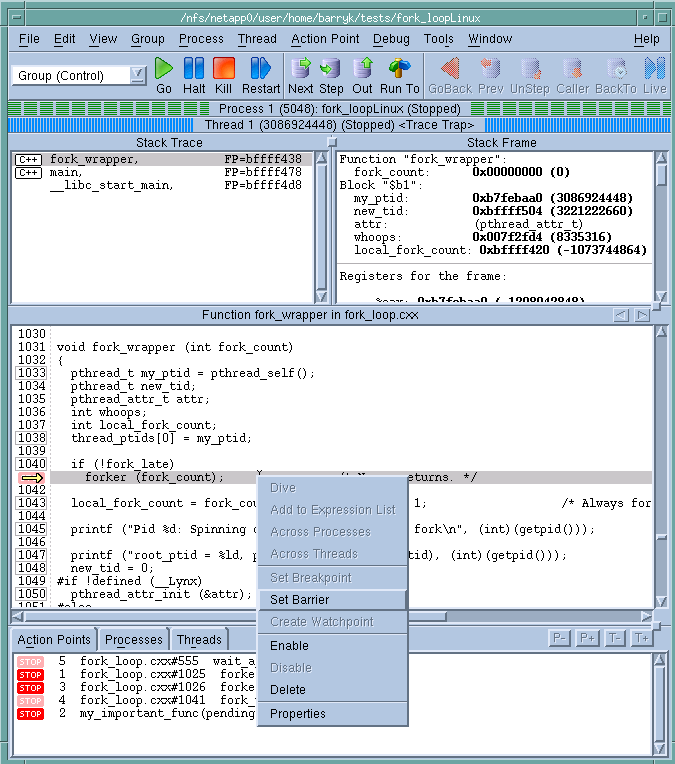
\includegraphics[height=0.75\textheight]{totalview-screenshot.png}

  \weblink{http://www.totalviewtech.com/products/totalview.html?via=rightbox}{TotalView}
  (Proprietary)
  \end{center}
\end{frame}
% -----------------------------------------------------------------------------
\begin{frame}{MPI Debuggers: DDT}
  \begin{center}
  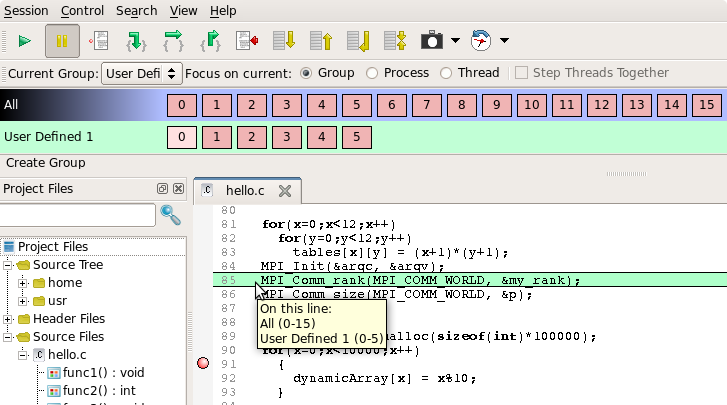
\includegraphics[width=\textwidth]{ddt-screenshot.png}

  Allinea \weblink{http://www.allinea.com/}{Distributed Debugging Tool}
  (Proprietary)
  \end{center}
\end{frame}
% -----------------------------------------------------------------------------
\begin{frame}{MPE/Jumpshot}
  \begin{center}
  \Huge MPE demo time
  \end{center}
\end{frame}
% -----------------------------------------------------------------------------
% TODO: collectives demo

% MPE, Jumpshot



\questionframe{}
%\imagecreditslide

\end{document}
% vim: foldmethod=marker

